\section{Le projet Comp@ssV4}

\subsection*{Préambule}

J'ai travaillé uniquement sur la partie qui concerne la migration et la nettoyage des données des clients dans le système SAP.
Le système SAP étant trop vaste, il m'est impossible de m'étendre sur tous les sujets. Je n'expliquerai donc dans ce rapport que les interactions à ce sujet.

Ce projet porte le nom de Comp@ssV4: \emph{Corporate Operationnal \& Management Performance @dvanced SyStem}.
Il succèdera à Comp@ssV2 et non à Comp@ssV3 qui fut un projet avorté et non poursuivi suite à un changement de politique interne.

\subsection{Une migration logicielle et architecturale}

Cette migration porte sur deux aspects :

\begin{itemize}
	\item Une mise à jour du logiciel.
	\item Un changement de l'architecture serveur (au regard des clients) pour une version plus unifiée.
\end{itemize}

\subsubsection{Mise à jour du logiciel}

Comme tout logiciel, il est maintenu pendant un certains temps. La version actuelle n'étant plus maintenue, il est nécessaire dans un environnement comme celui de Valeo de mettre à jour son système afin de réduire ses coûts de maintenance.

\subsubsection{Changement de l'architecture serveur}

En plus de la mise à niveau du logiciel SAP, Valeo a décidé de revoir entièrement son architecture applicative SAP et plus spécialement celle des clients.
Une vision plus unifiée et plus centralisée a été pensée et mise en place afin de correspondre aux exigences de la nouvelle politique du Groupe Valeo.
\clearpage

\subsubsection{Ancienne Structure: Comp@ssV2}

L'architecture de Comp@ssV2 peut être décrite comme ceci : 

 \begin{figure}[H]
    \centering
    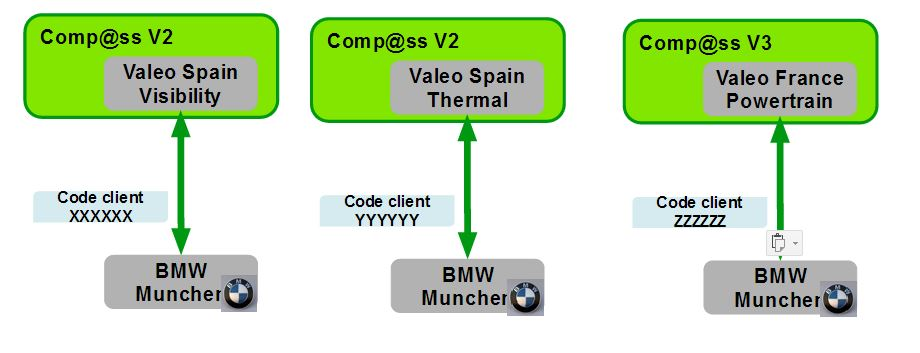
\includegraphics[height=7cm]{compassV2Customer.jpg}
	\caption{Structure du système Comp@ssV2 - Pas de référentiel client}\label{image.compassV2Customer} 
\end{figure}

\subsubsection{Nouvelle Structure: Comp@ssV4}

L'architecture de Comp@ssV4 peut être décrite comme ceci : 

 \begin{figure}[H]
    \centering
    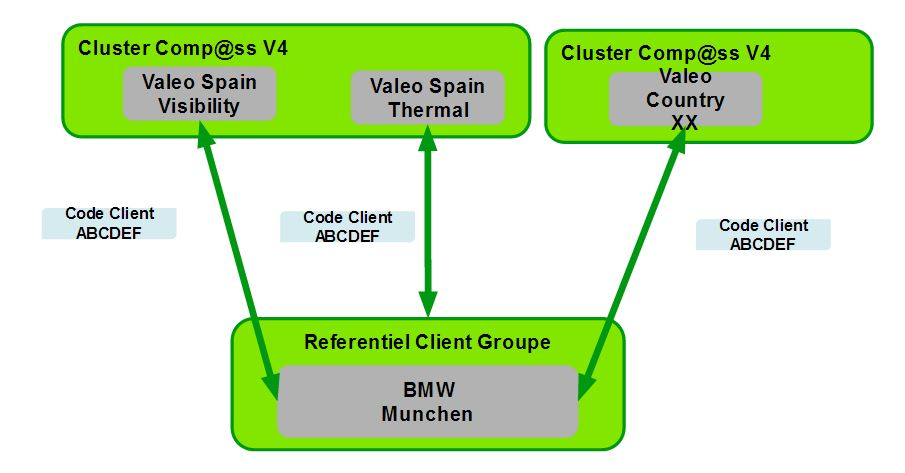
\includegraphics[height=9cm]{compassV4Customer.jpg}
	\caption{Structure du système Comp@ssV4 - Présence d'un référentiel client Groupe}\label{image.compassV4Customer} 
\end{figure}

\clearpage

\subsubsection{Résumé de la migration}

Ainsi, c'est une migration biaxiale qui est en cours de réalisation.\\
Cependant, la partie logicielle n'étant pas de notre périmètre, je ne m'étendrai pas sur ce sujet.

Ainsi, pour résumer, il est établi que toutes les machines SAP de Valeo pointeront vers un annuaire SAP de clients.\\ Ainsi chaque site aura une codification unifiée et cohérente avec les autres.
Le client numéro 1 sera le même quelque soit le système SAP de Valeo.

 \begin{figure}[H]
    \centering
    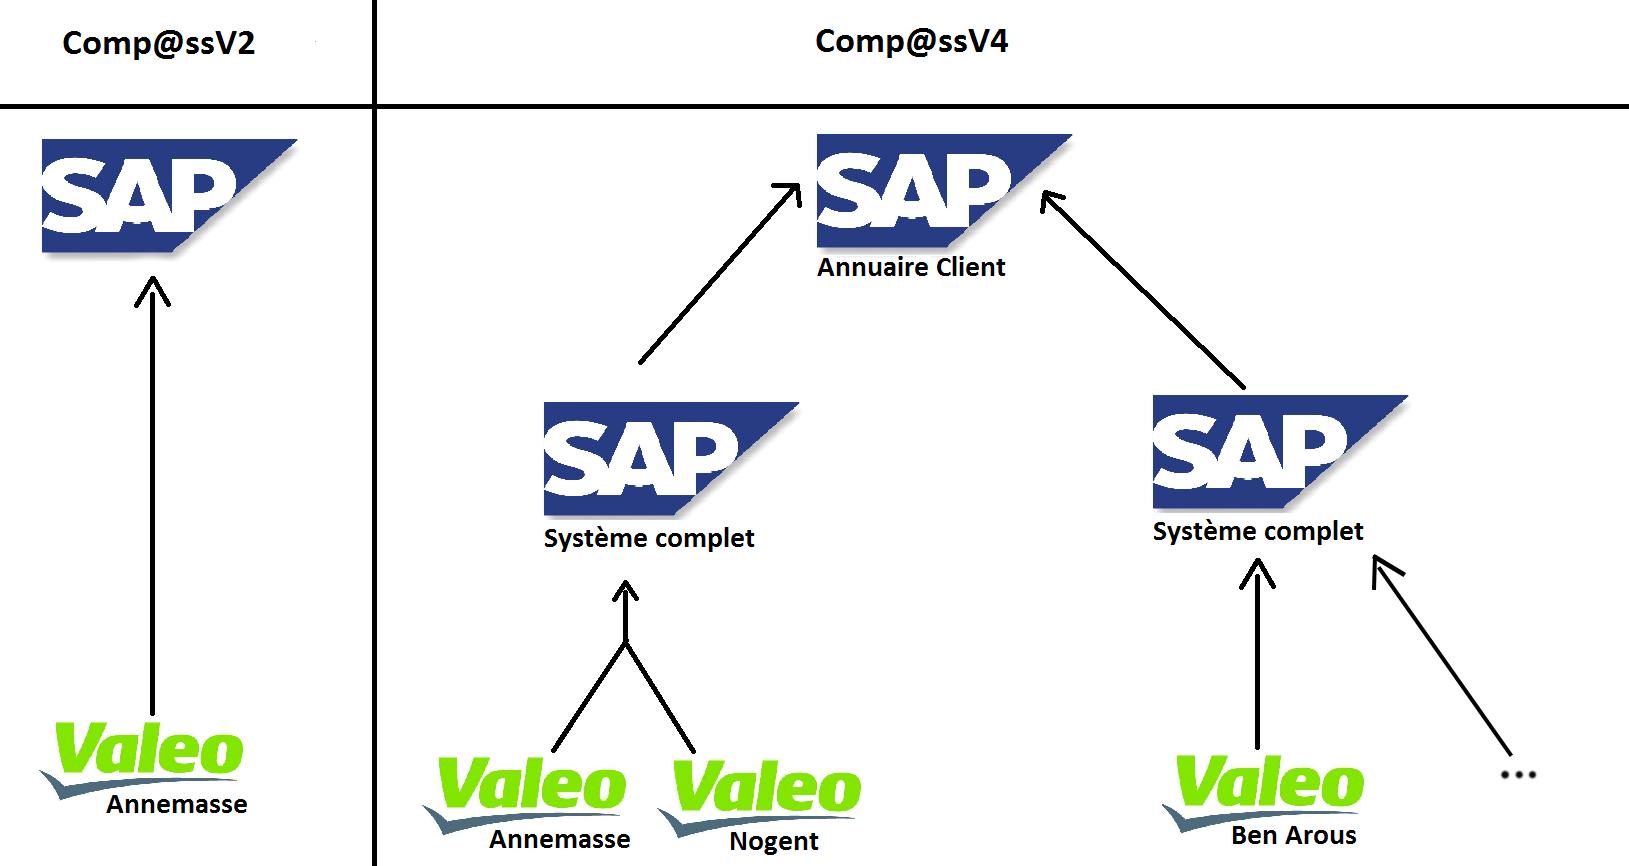
\includegraphics[height=10cm]{compassNewOrga.png}
	\caption{Comp@ssV2 vs Comp@ssV4 - Nouvelle Architecture Client}\label{image.compassNewOrga} 
\end{figure}
\textbf{
Les avantages d'une telle structure sont:}

\begin{itemize}\itemsep7pt
	\item Avoir une codification commune à tout le groupe Valeo. 
	\item Faciliter la comparaison entre les prévisions et les ventes réelles. 
	\item Faciliter la communication entre les sites Valeo. 
	\item Avoir une autorité commune sur un annuaire client unifié.
	\item Être capable de consolider le changement et les modifications des clients au niveau mondial.
	\item Avoir une vue globale du Business réalisé avec un client.
\end{itemize}

\clearpage